\section{Editing a Data Package} \label{sec:editing}

Once a data package has been created, you can edit its documentation in
one of the following ways: 

\begin{itemize}
  \setlength{\parskip}{1pt}
  \item using the Documentation menu items (for most editing)
  \item using the Morpho Editor 
\end{itemize}

Either tool permits you to change or delete documentation entered using
the Data Package wizard (or added to the data package in some other
way). The Morpho Editor can be used to add additional kinds of
documentation that are not included in the
\hyperref[sec:wizard-newdp]{Data Package wizard}, but you will most
often use the Documentation menu items. In this section, we will look at
both the \hyperref[sec:edit-doc-panels]{Documentation menu items} and
the \hyperref[sec:edit-doc-tree]{Morpho Editor} and how you can use them
to modify documentation. 

\subsection{Using the Documentation Menu} \label{sec:edit-doc-panels}

The Documentation menu (\autoref{fig:edit-documentation}) is activated
when the Morpho user opens an existing data package. The menu items
invoke editing tools and/or data entry screens that, together, enable
the user to edit any field in the data package documentation. 

The first menu item, ``Add/Edit Documentation'' opens the Morpho Editor
(described in \autoref{sec:edit-doc-tree}). The other menu items open
editable form views of specific subsections of the documentation
(\autoref{tab:edit-doc-items}). The form views are the same as the ones
used in the Data Package Wizard to create a new data package. For more
information about the fields in each editing screen, please see
\autoref{sec:adding-metadata}.

\begin{figure}
  \centering
    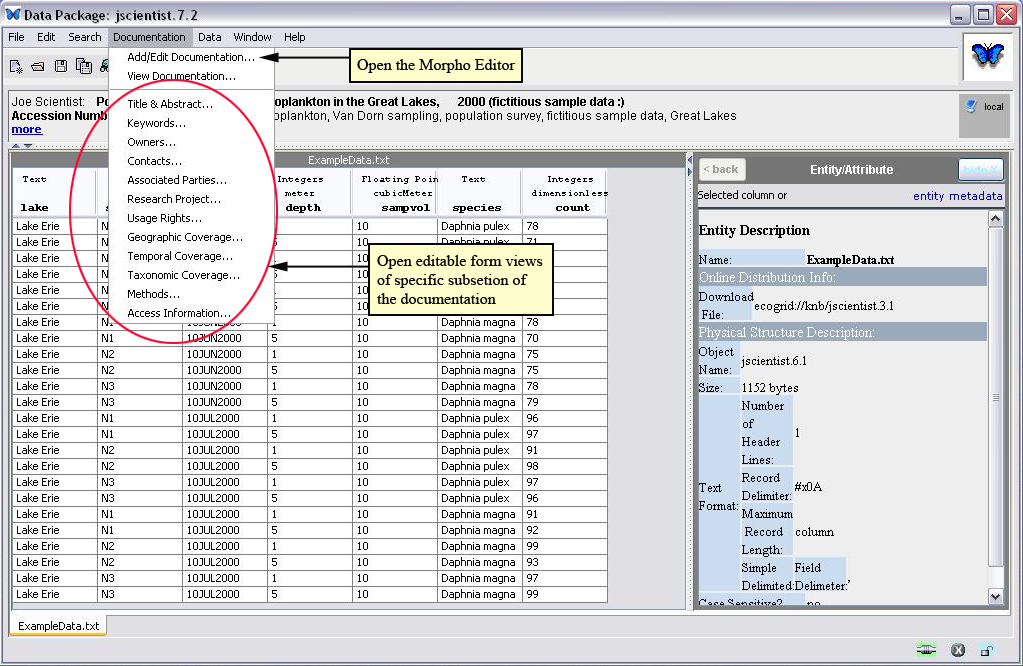
\includegraphics[width=0.7\textwidth]{images/edit-documentation.jpg}
  \caption{The Documentation menu items become active when a user opens
    an existing data package.}
  \label{fig:edit-documentation}
\end{figure}

\begin{table}[htbp]
  \centering
  \begin{tabular}{|c|m{0.7\textwidth}|}
  \hline
  \textbf{Menu Item} & \textbf{Description} \\
  \hline
  Add/Edit Documentation &
    Invoke the full-featured \hyperref[sec:edit-doc-tree]{Morpho
    Editor}, which provides editing access to all documentation fields
    in the data package. Note that the Editor is rarely required as most
    editing is done with the other options in the menu. \\
  \hline
  View Documentation &
    View all data package documentation in one window. \\
  \hline
  Title \& Abstract &
    Modify the \hyperref[sec:wizard-dp-title]{data package title and
    abstract}. \\
  \hline
  Keywords &
    Modify the \hyperref[sec:wizard-dp-keywords]{keywords} (the significant
    words or phrases) that help identify the data set. \\
  \hline
  Owners &
    Modify the name or contact information of the
    \hyperref[sec:wizard-dp-people]{data package owner}. \\
  \hline
  Contacts &
    Modify the name or contact information of the
    \hyperref[sec:wizard-dp-people]{data package contact}. \\
  \hline
  Associated Parties &
    Modify the name or contact information for any
    \hyperref[sec:wizard-dp-people]{parties associated} with the data
    package. \\
  \hline
  Research Project &
    Indicate whether or not the data package is part of a larger
    \hyperref[sec:wizard-dp-project]{research project}. \\
  \hline
  Usage Rights &
    Modify the \hyperref[sec:wizard-dp-usage]{usage rights} for the data
    package. \\
  \hline
  Geographic Coverage &
    Modify the \hyperref[sec:wizard-dp-coverage]{geographic coverage} of
    the data package. \\
  \hline
  Temporal Coverage &
    Modify the \hyperref[sec:wizard-dp-coverage]{temporal coverage} of
    the data package. \\
  \hline
  Taxonomic Coverage &
    Modify the \hyperref[sec:wizard-dp-coverage]{taxonomic coverage} of
    the data package. \\
  \hline
  Methods &
    Modify the \hyperref[sec:wizard-dp-methods]{methods and sampling
    design} documentation. \\
  \hline
  Access Permissions &
    Modify the \hyperref[sec:wizard-dp-access]{access} rights granted
    to individuals and the public. \\
  \hline
  Replication Policy &
    Modify the \hyperref[sec:wizard-dp-replication]{replication} policy
    for the object. \\  
  \hline
  \end{tabular}
  \caption{Documentation menu items.}
  \label{tab:edit-doc-items}
\end{table}

\subsection{Using the Morpho Editor} \label{sec:edit-doc-tree}

Most editing is done with the options in the documentation menu.
However, if there is a metadata field that is not included in the
Documentation menus, you can use the Morpho Editor to access and modify
it. The editor displays each module (the items describing the data
package, such as its creator, usage rights, and documented data tables)
so that users can select, display, and modify the content associated
with each.

To open the Morpho Editor (\autoref{fig:tree-editor}), open the data
package you wish to edit and then do one of the following:
\begin{itemize}
  \setlength{\parskip}{1pt}
  \item select ``Add/Edit Documentation'' from the Documentation menu,
  \item right-click a data table or other data object within the data
    package, and choose ``Add Documentation''. 
\end{itemize}

\begin{figure}
  \centering
    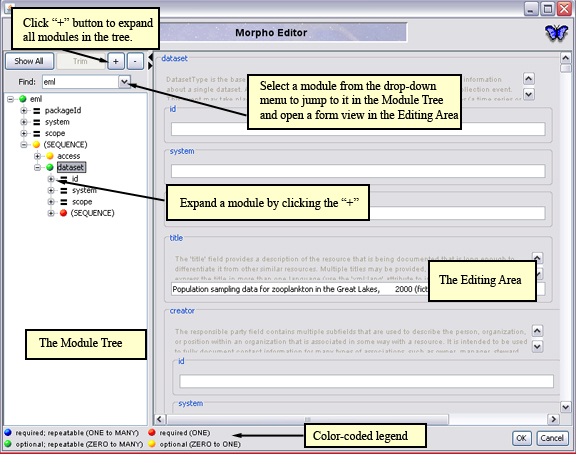
\includegraphics[width=0.7\textwidth]{images/tree-editor.jpg}
  \caption{The Morpho Editor.}
  \label{fig:tree-editor}
\end{figure}

The editor consists of two panels: the Module Tree (on the left) and the
Editing Area (on the right). Click the ``+'' symbol next to each module
to browse through the hierarchy (or use the scrollbar on the right side
of the editing area to scroll through displayed fields). To expand and
view all levels of the module tree, click on the ``+'' button at the top
of the tree. 

Initially, the Editor displays only the modules that already exist in
the data package documentation. To view a module, select the module by
clicking it. The Editor then displays a form-based view of the
information contained in the selected module. To edit the content of a
field, click the field and enter text. The 'tab key' moves the selection
to the next editable field. 

To add documentation for modules that are not initially displayed in the
Module Tree, click the ``Show All'' button. The Morpho Editor displays
all modules in the tree. To return to the original view, click ``Trim.'' 

You can also open modules using the Find drop-down menu at the top of
the Module Tree. For example, to edit documentation for a data table,
select ``dataTable'' from the Find menu. The Morpho Editor expands the
dataTable module. If the data package contains several data tables,
select the one you wish to edit. Use the scroll bar at the right of the
screen to scroll through the table attributes, or select
``attributeList'' from the Find menu to display the attributes in the
module tree.

Modules are color-coded to indicate which are required and which are
repeatable. Blue and red nodes are required. Green and yellow nodes are
optional. Blue and green nodes are repeatable, meaning they can be
duplicated (for example, you can specify multiple data set owners). Red
nodes can be used only once, and yellow nodes can be used once or not at
all (zero). The Morpho Editor includes a legend in the lower-left
corner.

Right-click any module in the Module Tree to display a popup menu
(\autoref{fig:tree-editor-actions}) containing options to duplicate,
delete, or copy and paste that module. Note that these operations affect
the selected module and all of its children. For example, if you choose
to duplicate the keywordSet module, you will also duplicate the keyword
modules that are nested inside it.

\begin{figure}
  \centering
    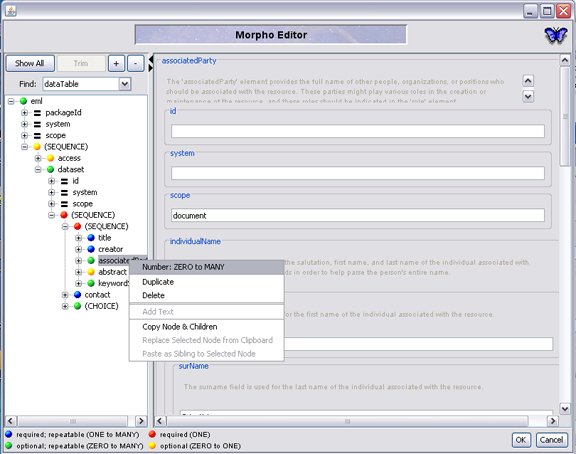
\includegraphics[width=0.7\textwidth]{images/tree-editor-actions.jpg}
  \caption{Right-click a module in the Module Tree to duplicate, delete,
    or copy that module and the modules nested inside it.}
  \label{fig:tree-editor-actions}
\end{figure}
